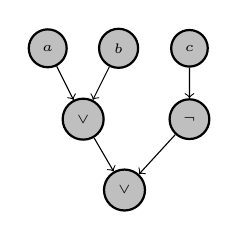
\begin{tikzpicture}[scale=0.3] % , baseline = -3.5pt



	\node [circle, draw, thick, fill=gray!50] (T1) at (0,0) {\tiny $a$};
	\node [circle, draw, thick, fill=gray!50] (T2) at (3,0) {\tiny $b$};
	\node [circle, draw, thick, fill=gray!50] (T3) at (6,0) {\tiny $c$};
	
	\node [circle, draw, thick, fill=gray!50] (and) at (1.5,-3) {\tiny $\lor$};
	\node [circle, draw, thick, fill=gray!50] (not) at (6,-3) {\tiny $\lnot$};	
	
	\draw [->] (T1) -- (and);
	\draw [->] (T2) -- (and);
	
	\draw [->] (T3) -- (not);	
	
	\node [circle, draw, thick, fill=gray!50] (head) at (3.25,-6) {\tiny $\lor$};
	
	\draw [->] (and) -- (head);
	\draw [->] (not) -- (head);			



\end{tikzpicture}